% begin module parametric-ex2
\begin{frame}
\begin{example}[Example 2, p. 658]
Sketch and identify the curve defined by the parametric equations
\abovedisplayskip=2pt
\belowdisplayskip=2pt
\[
\alert<handout:0| 15>{x = \cos t}, \qquad \alert<handout:0| 14>{y = \sin t}.
\]
\begin{columns}[c]
\column{.55\textwidth}

\ \only<handout:0| -2>{%
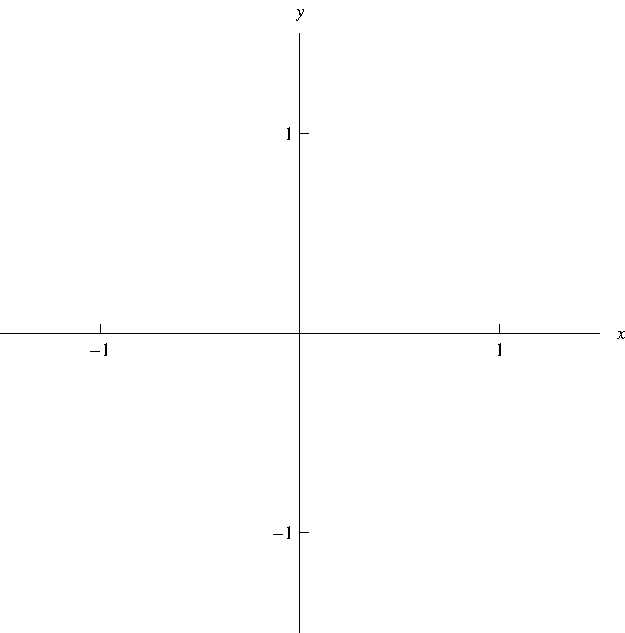
\includegraphics[height=6cm]{parametric-curves/pictures/11-01-ex2a.pdf}%
}%
\only<handout:0| 3-4>{%
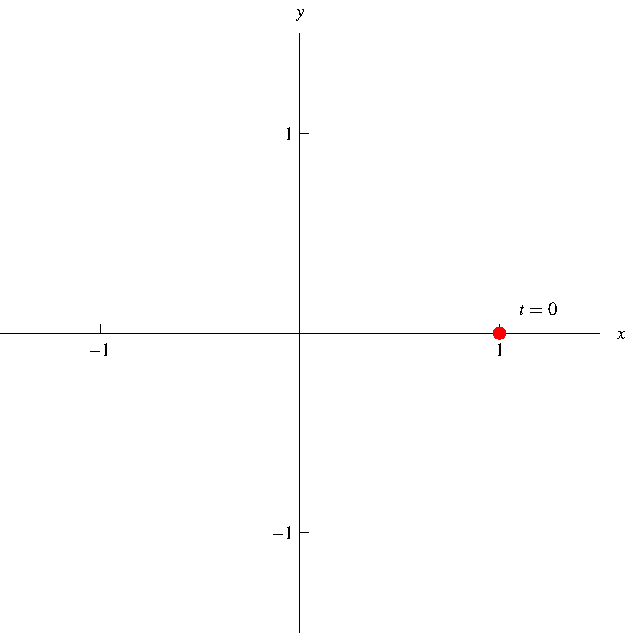
\includegraphics[height=6cm]{parametric-curves/pictures/11-01-ex2b.pdf}%
}%
\only<handout:0| 5-6>{%
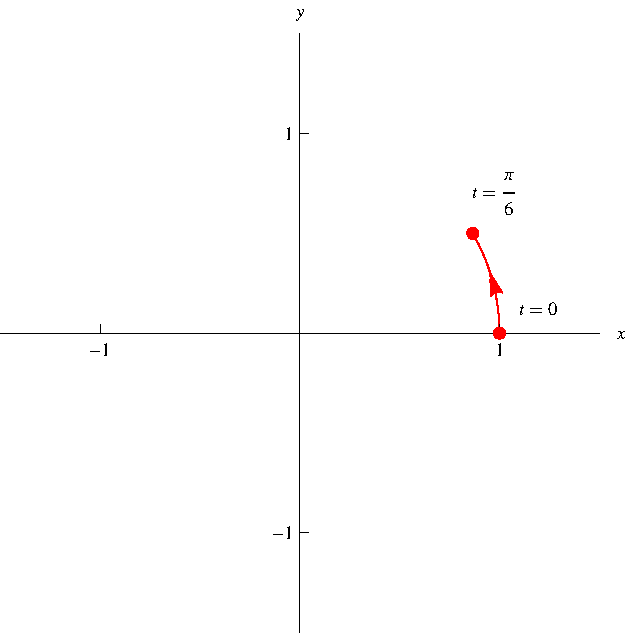
\includegraphics[height=6cm]{parametric-curves/pictures/11-01-ex2c.pdf}%
}%
\only<handout:0| 7-8>{%
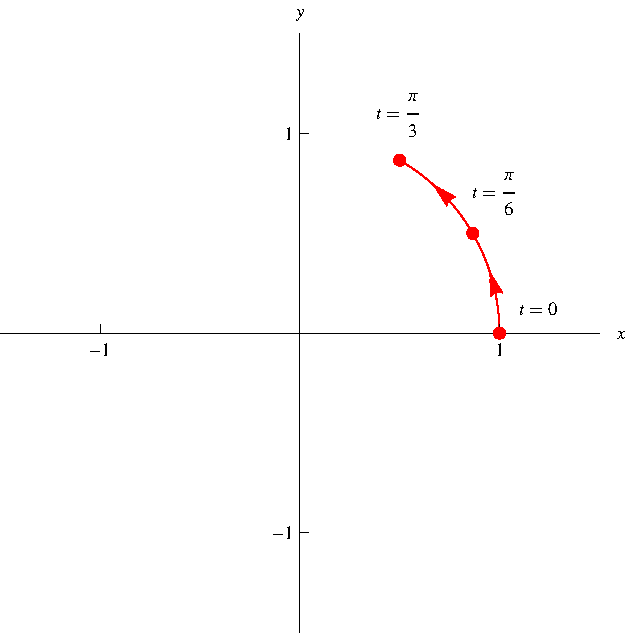
\includegraphics[height=6cm]{parametric-curves/pictures/11-01-ex2d.pdf}%
}%
\only<handout:0| 9-10>{%
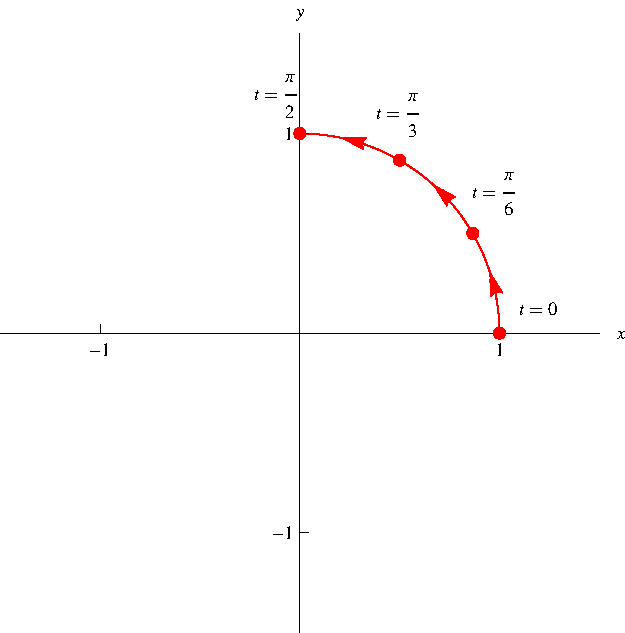
\includegraphics[height=6cm]{parametric-curves/pictures/11-01-ex2e.pdf}%
}%
\only<handout:0| 11-12>{%
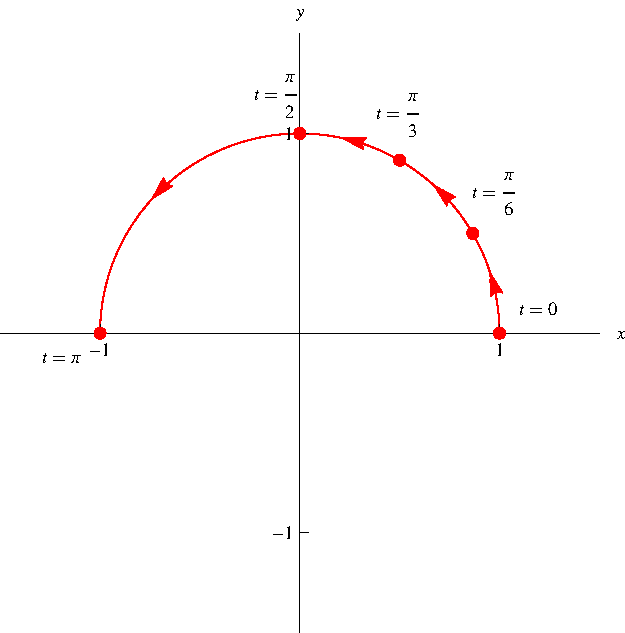
\includegraphics[height=6cm]{parametric-curves/pictures/11-01-ex2f.pdf}%
}%
\only<handout:0| 13-14>{%
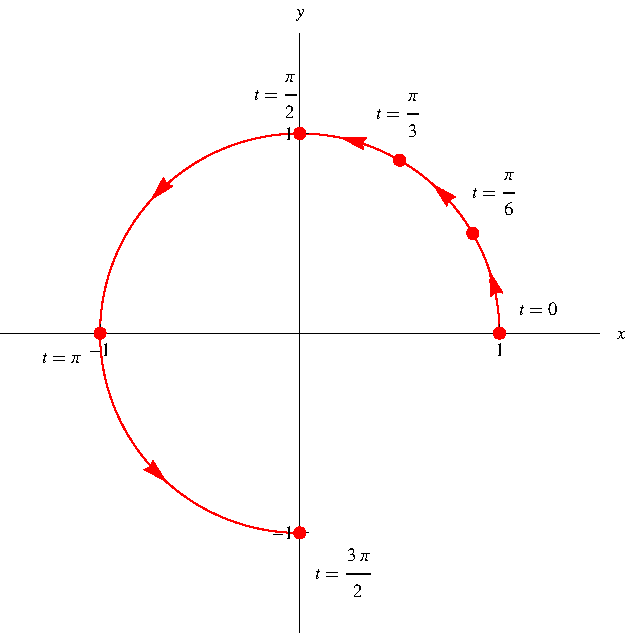
\includegraphics[height=6cm]{parametric-curves/pictures/11-01-ex2g.pdf}%
}%
\only<15->{%
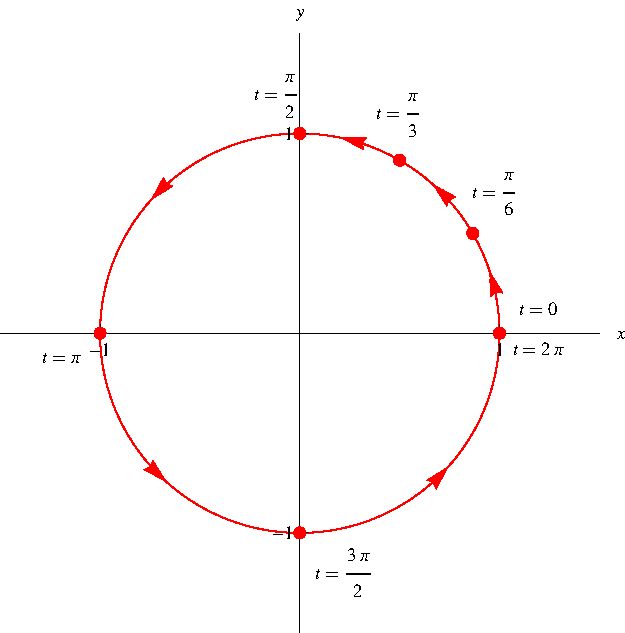
\includegraphics[height=6cm]{parametric-curves/pictures/11-01-ex2h.pdf}%
}%

\column{.45\textwidth}
\[
\begin{array}{|r|r|r|}
\hline
t & x & y\\
\hline
\alert<handout:0| 2-3>{0} &%
\alert<handout:0| 2-3>{\uncover<3->{1}} &%
\alert<handout:0| 2-3>{\uncover<3->{0}} \\%
\alert<handout:0| 4-5>{\pi / 6} &%
\alert<handout:0| 4-5>{\uncover<5->{\sqrt{3}/ 2}} &%
\alert<handout:0| 4-5>{\uncover<5->{1/2}} \\%
\alert<handout:0| 6-7>{\pi / 3} &%
\alert<handout:0| 6-7>{\uncover<7->{1/2}} &%
\alert<handout:0| 6-7>{\uncover<7->{\sqrt{3}/2}} \\%
\alert<handout:0| 8-9>{\pi /2} &%
\alert<handout:0| 8-9>{\uncover<9->{0}} &%
\alert<handout:0| 8-9>{\uncover<9->{1}} \\%
\alert<handout:0| 10-11>{\pi} &%
\alert<handout:0| 10-11>{\uncover<11->{-1}} &%
\alert<handout:0| 10-11>{\uncover<11->{0}} \\%
\alert<handout:0| 12-13>{3\pi/2} &%
\alert<handout:0| 12-13>{\uncover<13->{0}} &%
\alert<handout:0| 12-13>{\uncover<13->{-1}} \\%
\alert<handout:0| 14-15>{2\pi} &%
\alert<handout:0| 14-15>{\uncover<15->{1}} &%
\alert<handout:0| 14-15>{\uncover<15->{0}} \\%
\hline
\end{array}
\]
\abovedisplayskip=2pt
\belowdisplayskip=2pt
\[
\uncover<16->{%
x^2 + y^2 = %
}%
\uncover<17->{%
\cos^2 t+ \sin^2 t = %
}%
\uncover<18->{%
1%
}%
\]
\uncover<19->{%
Therefore $(x,y)$ travels on the unit circle $x^2 + y^2 = 1$.
}%
\end{columns}
\end{example}
\end{frame}
% end module parametric-ex2
